\chapter{Introduction et motivation}
\label{chap-intro}
L'oxalate de calcium est un matériau très présent dans la nature.
Notamment, on peut le retrouver dans les calculs rénaux
(communément appelés ``pierres aux reins'', cf. \cref{fig-calcul})
qui sont formés par le phosphalte de calcium,
une plus grande structure qui contient les états hydratés de l'oxalate de calcium.
Pour étudier un tel matériau sans changer sa structure ou le détruire,
on fait souvent des études spectroscopiques.
Cela consiste à étudier les propriétés optiques et diélectriques du matériau en
analysant la réponse du matériau à une perturbation externe.
Typiquement, on peut déduire des spectroscopies de perte et d'absorption
à partir de la fonction diélectrique du matériau.

Dans le cadre du projet de recherche en laboratoire de l'École Polytechnique,
nous avons choisi d'aborder le sujet (parmi d'autre) proposé par M. Franceso Sottile
du Laboratoire des Solides Iradiés de l'École Polytechnique (LSI).
Ce travail consiste à évaluer les propriétés spectroscopiques de l'oxalate de calcium par des calculs \textit{ab initio}.
Il s'agit donc de bien comprendre la théorie de la fonctionnelle de la densité
(\textit{Density Functional Theory}, DFT)
et la théorie de la fonctionnelle de la densité dépendante du temps
(\textit{Time-Dependent Density Functional Theory}, TDDFT)
et de les appliquer avec les codes existants.
La DFT et la TDDFT sont deux pilliers des calculs \textit{ab initio}
qui donnent des bonnes prédictions théoriques par rapport aux expériences réelles.

L'intérêt de ce projet de recherche est de fournir une prédiction théorique et numérique
sur les caractéristiques de l'oxalate de calcium,
surtout pour une comparaison avec des études expérimentaux qui est aujourd'hui en cours
au Laboratoire de Physique des Solides (LPS) à Orsay.

La stratégie du projet est d'abord de trouver l'état fondamental du système étudié,
et ensuite de calculer les propriétés diélectriques.
Le reste de ce rapport est organisé de la façon suivante:
Le \cref{chap-theory} est consacré à la description des méthodes de calcul
(DFT statique pour l'état fondamental et TDDFT pour les propriétés diélectriques).
Les méthodes d'approximation engagées dans la simulation sont présentées dans le \cref{chap-simulation}.
Les résultats obtenus sont illustrés dans le \cref{chap-results}.
\begin{figure}[h!]
  \vspace{6pt} 
  \centering
  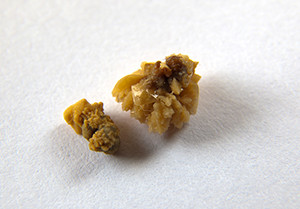
\includegraphics[width=\textwidth]{calcium-oxalate-kidney-stone}
  \caption{Calculs rénaux, communément appelés ``pierres aux reins''}\label{fig-calcul}
\end{figure}
